\section{Durchführung}
\label{sec:Durchführung}

\subsection{Kalibrierung des Reflexklystrons und der Messleitung}
\label{ssec:Kalibrierung}

Zur Kalibrierung des Klystrons wird ein Aufbau wie in \autoref{fig:aufbau1} verwendet.

\begin{figure}
    \centering
    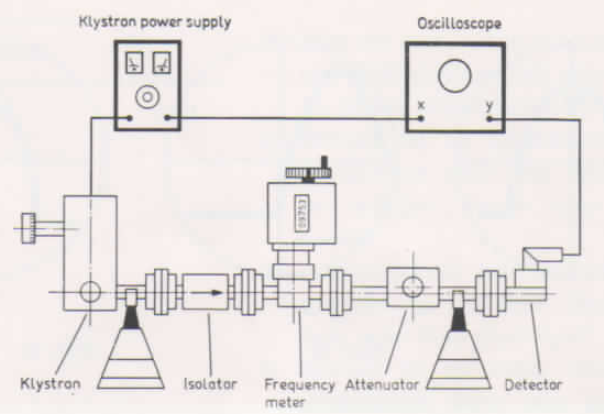
\includegraphics[width=0.7\textwidth]{images/aufbau1.png}
    \caption{Aufbau für Klystron-Untersuchungen mit dem Osszilloskop \cite{V53_old}}
    \label{fig:aufbau1}
\end{figure}

Zunächst muss an das Reflexklystron eine $\SI{6.3}{\volt}$ Heizspannung angelegt werden und gewartet werden bis sich die Temperatur stabilisiert hat.
Das Dämpfungsglied wird auf $\SI{30}{\decibel}$, die Resonatorspannung auf $\SI{300}{\volt}$ und die Reflektorspannung auf $\SI{200}{\volt}$ gestellt.
Nun wird am Speisegerät eine Sinusmodulation von $\SI{50}{\hertz}$ mit einer $\SI{85}{\volt}$ Amplitude eingeschaltet.

Nun ist auf dem Oszilloskop auf der $x$-Achse eine Sinusspannung und auf der $y$-Achse das Detektorsignal angezeigt.
Es sollten die Ablenkkoeffizienten so eingestellt werden, dass das ganze Bild zu sehen ist, 
außerdem muss das Bild horizontal zentriert werden, damit in der Mitte genau die eingestellte Reflektorspannung liegt.

Auf dem Oszilloskop sollte nun annähernd eine Parabel wie in \autoref{fig:modulation} zu sehen sein.
Diese Parabel kann nun vermessen werden, indem der Wert der Reflektorspannung verändert und notiert wird, 
sodass nacheinander in der Mitte des Oszilloskops das linke Ende, das Maximum und das rechte Ende zu sehen sind.
Die Amplitude der Parabel kann auf dem Oszilloskop abgelesen werden.

Zusätzlich kann mit dem Frequenzmesser die Resonanzfrequenz des Klystrons je nach Reflektorspannung bestimmt werden,
indem der Frequenzmesser so angepasst wird, das der dadurch entstandene \enquote{dip} auf dem Maximum der Parabel liegt.

Auf diese Weise werden die ersten drei Moden des Reflexklystrons vermessen.

\begin{figure}
    \centering
    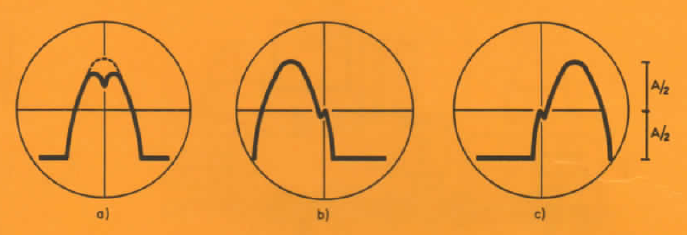
\includegraphics[width=0.8\textwidth]{images/frequenz_dip.png}
    \caption{Resultierender \enquote{dip} mit angepasstem Frequenzmesser \cite{V53_old}}
    \label{fig:frequenz_dip}
\end{figure}

Außerdem werden für den Modus, der am nächsten an $\SI{200}{\volt}$ Reflektorspannung liegt, mit dem Frequenzmesser die Punkte halber Leistung bestimmt,
indem auf dem Oszilloskop Bilder wie in \autoref{fig:frequenz_dip} erzeugt werden und Frequenz und Reflektorspannung abgelesen werden.

\subsection{Messung der Frequenz, Wellenlänge und Dämpfung auf dem Hohlleiter}
\label{ssec:Messung_Hohlleiter}

Für die Messung der Frequenz, der Wellenlänge und der Dämpfung der Hohlleiterwellen wird ein Aufbau wie in \autoref{fig:aufbau2} verwendet.
Für die Frequenz- und Dämpungs-Messung wird am Ende ein Abschluss verwendet und für die Wellenlängen-Messung wird ein einstellbarer Kurzschluss verwendet.

\begin{figure}
    \centering
    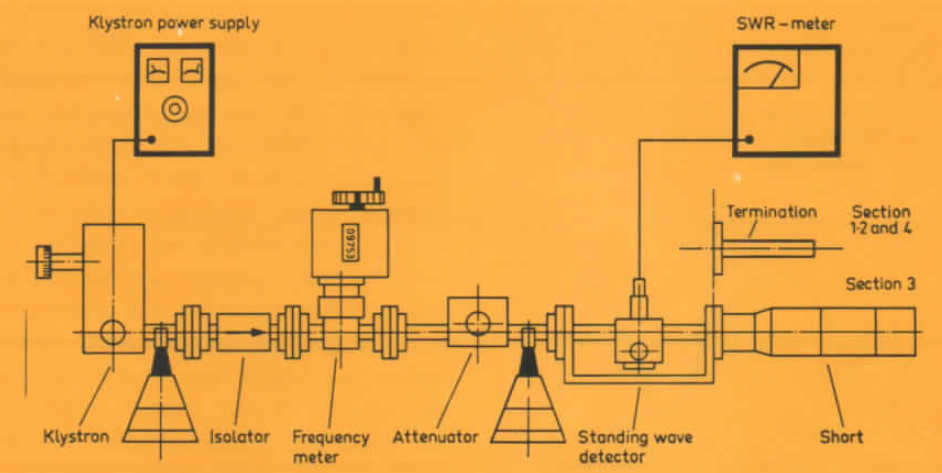
\includegraphics[width=0.7\textwidth]{images/aufbau2.png}
    \caption{Aufbau zur Frequenz-, Wellenlängen- und Dämpungs-Messung \cite{V53_old}}
    \label{fig:aufbau2}
\end{figure}

Es wird eine Dämpfung von $\SI{20}{\decibel}$ eingestellt und die Mode um $\SI{200}{\volt}$ Reflektorspannung eingestellt, sodass auf dem SWR-Messer ein Maximum zu sehen ist.
Das Klystron wird mit einer Rechteckspannung moduliert.

Nun wird der Frequenzmesser so eingestellt, dass ein \enquote{dip} zu erkennen ist.
Die Frequenz kann abgelesen und notiert werden.
Danach wird der Frequenzmesser wieder verstimmt.

Für die Wellenlängen-Messung wird die Messsonde verschoben und der Abstand zweier aufeinanderfolgender Minima wird notiert.
Außerdem werden nun die Innenmaße des Hohlleiters benötigt.

Für die Dämpfungs-Messung wird die Dämpfung auf die maximale darstellbare Dämpfung auf dem SWR-Meter im $\SI{30}{\decibel}$ Modus eingestellt.
Nun wird die Millimeterschraube des Dämpfungsglieds so verstellt, dass die Dämpfung auf dem SWR-Meter um $\SI{2}{\decibel}$ sinkt.
Die Einstellung der Millimeterschraube wird zusammen mit der Dämpfung notiert.
Dies wird so lange wiederholt, bis die Dämpfung nicht mehr ablesbar ist.

\subsection{Messung des Stehwellenverhältnisses}
\label{ssec:Messung_SWR}

Für die Stehwellenverhältnis-Messung werden die drei, in der Theorie beschriebenen, Messmethoden verwendet.
Aber für alle dieser Methoden wird ein Aufbau wie in \autoref{fig:aufbau3} verwendet.

\begin{figure}
    \centering
    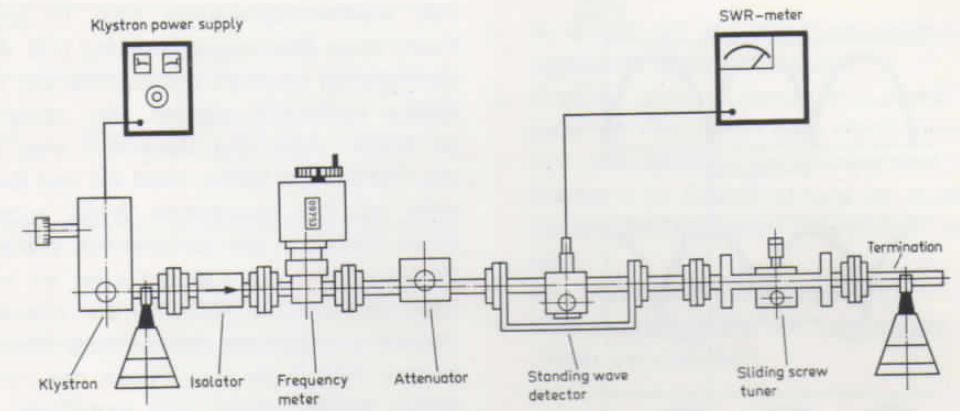
\includegraphics[width=0.7\textwidth]{images/aufbau3.png}
    \caption{Aufbau zur Stehwellenverhältnis-Messung \cite{V53_old}}
    \label{fig:aufbau3}
\end{figure}

Auch hier wird eine Dämpfung von $\SI{20}{\decibel}$ verwendet und das Klystron bei der gleichen Mode rechteckmoduliert.
Die Verschiebung der Sonde sollte nun den Ausschlag des SWR nur wenig verändern.

Für die Direkte Messung wird die Sonde des Gleitschraubentransformators in die Messleitung gedreht.
Die Sonde wird zu einem Maximum geführt und das SWR-Meter wird auf das Maximum gestellt.
Nun wird die Sonde zum nächsten Minimum geführt und auf dem SWR-Meter kann das Stehwellenverhältnis abgelesen werden.
Dies wird für insgesamt 4 verschiedene Sondentiefen ($3,5,7,\SI{9}{\milli\meter}$) durchgeführt.

Für die $\SI{3}{\decibel}$-Messung wird der Gleitschraubentransformator auf $\SI{9}{\milli\meter}$ gestellt.
Das SWR-Meter wird an einem Minimum auf $\SI{3}{\decibel}$ gestellt
und es werden die Punkte links und rechts gesucht, an denen das SWR-Meter den Vollausschlag erreicht.
Außerdem wird mit einem Kurzschluss statt Gleitschraubentransformator und Abschluss der Abstand zweier Minima gemessen.

Für die Abschwächer-Messung wird wieder der Gleitschraubentransformator auf $\SI{9}{\milli\meter}$ gestellt.
Die Sonde wird auf ein Minimum geführt,
bei einer eingestellten Dämpfung (z.B. $\SI{20}{\decibel}$) wird das SWR-Meter auf einen gut ablesbaren Wert gestellt (z.B. $\SI{3}{\decibel}$). 
Dann wird ein Maximum gesucht und gleichzeitig die Dämpfung verändert. 
An dem Maximum sollte die Dämpfung so eingestellt werden, dass der gleiche Wert auf dem SWR-Meter angezeigt wird wie zuvor beim Minimum.
Die beiden eingestellten Dämpfungen werden notiert.